% This file was created with tikzplotlib v0.10.1.post9.
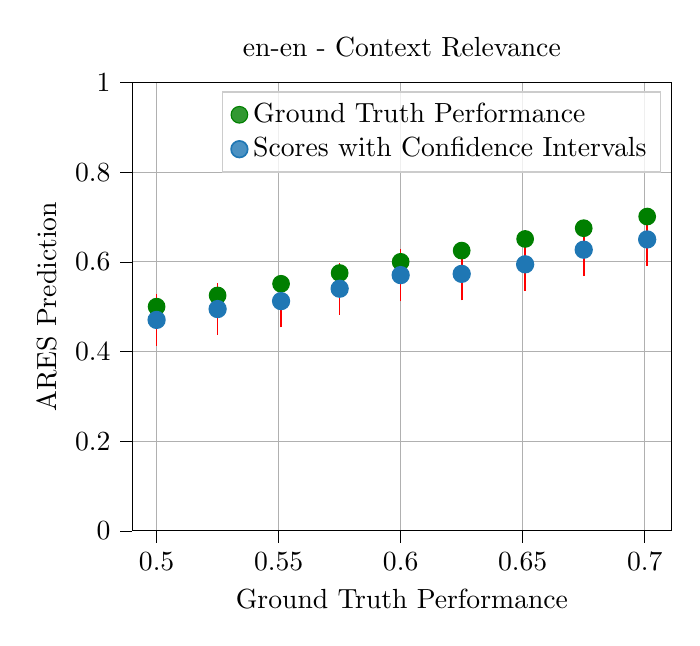
\begin{tikzpicture}

\definecolor{darkgrey176}{RGB}{176,176,176}
\definecolor{green01270}{RGB}{0,127,0}
\definecolor{lightgrey204}{RGB}{204,204,204}
\definecolor{steelblue31119180}{RGB}{31,119,180}

\begin{axis}[
legend cell align={left},
legend style={
  fill opacity=0.8,
  draw opacity=1,
  text opacity=1,
  draw=lightgrey204,
  mark options={mark size=3}
},
tick align=outside,
tick pos=left,
title={en-en - Context Relevance},
x grid style={darkgrey176},
xlabel={Ground Truth Performance},
xmajorgrids,
xmin=0.48995, xmax=0.71105,
xtick style={color=black},
y grid style={darkgrey176},
ylabel={ARES Prediction},
ymajorgrids,
ymin=0, ymax=1,
ytick style={color=black}
]
\addplot [draw=green01270, fill=green01270, mark size=3pt, mark=*, only marks]
table{%
x  y
0.5 0.5
0.525 0.525
0.551 0.551
0.575 0.575
0.6 0.6
0.625 0.625
0.651 0.651
0.675 0.675
0.701 0.701
};
\addlegendentry{Ground Truth Performance}
\path [draw=red, semithick]
(axis cs:0.5,0.413)
--(axis cs:0.5,0.528);

\path [draw=red, semithick]
(axis cs:0.525,0.437)
--(axis cs:0.525,0.553);

\path [draw=red, semithick]
(axis cs:0.551,0.454)
--(axis cs:0.551,0.571);

\path [draw=red, semithick]
(axis cs:0.575,0.482)
--(axis cs:0.575,0.598);

\path [draw=red, semithick]
(axis cs:0.6,0.512)
--(axis cs:0.6,0.629);

\path [draw=red, semithick]
(axis cs:0.625,0.514)
--(axis cs:0.625,0.632);

\path [draw=red, semithick]
(axis cs:0.651,0.535)
--(axis cs:0.651,0.654);

\path [draw=red, semithick]
(axis cs:0.675,0.568)
--(axis cs:0.675,0.686);

\path [draw=red, semithick]
(axis cs:0.701,0.591)
--(axis cs:0.701,0.709);

\addplot [semithick, steelblue31119180, mark=*, mark size=3, mark options={solid}, only marks]
table {%
0.5 0.470380667236955
0.525 0.494646600778676
0.551 0.512362637362637
0.575 0.539999179924553
0.6 0.570380667236955
0.625 0.573145175673266
0.651 0.594480519480519
0.675 0.627021563342318
0.701 0.649925074925075
};
\addlegendentry{Scores with Confidence Intervals}
\end{axis}

\end{tikzpicture}
